%!TEX root=../Vorlage_DA.tex
%	########################################################
% 				Allgemeiner Teil (Theorie)
%	########################################################


%	--------------------------------------------------------
% 	Sprachspezifikation
%	--------------------------------------------------------
\newpage
\section{Sprachspezifikation}

\subsection{Pr\"aprozessor}

Der Pr\"aprozessor erm\"oglicht die Nutzung mehrer Dateien und verf\"ugt \"uber die Funktion einzelne Codeteile zu deaktivieren, wie es auch in C der Fall ist. Pr\"aprozessorargumente beginnen dabei jeweils mit einem Hashtag, gefolgt von der jeweiligen Direktive und teilweise einem oder mehreren Argumenten.

\subsubsection{\#include Direktive}

Mithilfe eines \textbf{\#include} k\"onnen andere Dateien eingebunden werden. Es gibt dabei 2 Arten von \textbf{\#include}, welche sich durch den jeweiligen Suchpfad unterscheiden. Aus technischer Sicht kopiert der Pr\"aprozessor die jeweilige Datei an die Stelle wo das \textbf{\#include} geschrieben ist.

\htlParagraph{Suche im Standard-Include-Pfad}

Der Standard-Include-Pfad stellt der Ordner clib dar, in welchem sich die Standardbibliothek befindet. Dieser befindet sich standardm\"a\ss{}ig im Hauptverzeichnis von C Compact.

\begin{lstlisting}[language=C]
#include <stdio.h>
\end{lstlisting}

\htlParagraph{Suche im aktuellen Verzeichnis}

Wenn selbst geschriebene Programmdateien eingebunden werden, wird der Pfad relativ zum aktuellen Verzeichnis angegeben. So ist es m\"oglich Programme zu entwickeln, welche aus mehrere Dateien nutzen.

\begin{lstlisting}[language=C]
#include "foo.cmm"
\end{lstlisting}

\subsubsection{\#define Direktive}

Es ist m\"oglich w\"ahrend des Pr\"aprozessorvorganges Variablen zu definieren, welche aber nur im Pr\"aprozessor ausgewertet werden k\"onnen. Es ist nicht m\"oglich mithilfe eines \textbf{\#define} Quelltext zu ver\"andern, wie es in C m\"oglich ist!

Es ist m\"oglich, einem Define einen Wert zuzuweisen, welcher eine Ganze Zahl sein muss. Falls kein Wert angegeben ist wird 1 angenommen.

\begin{lstlisting}[language=C]
#define __DEFINE_WITHOUT_VALUE__
#define __DEFINE_WITH_VALUE__ 0
\end{lstlisting}

Falls ein \textbf{\#define} mit dem gleichen Namen bereits existiert, wird dieses \"uberschrieben.

\subsubsection{\#undef Direktive}

Mithilfe eines \textbf{\#undef} kann eine definierte Variable gel\"oscht werden. Die Variable steht somit nicht mehr zur Verf\"ugung, bis die Variable erneut definiert wird.

\begin{lstlisting}[language=C]
#undef __DEFINE_WHICH_IS_NOW_DELETED__
\end{lstlisting}

\subsubsection{\#ifdef, \#ifndef, \#else und \#endif Direktive}

Es ist m\"oglich abzufragen, ob es eine bestimmte Variablendefinition gibt oder nicht gibt. Diese Abfrage wird mit den Pr\"aprozessorargumenten \textbf{\#ifdef} bzw. \textbf{\#ifndef} eingeleitet, und muss mit einem \textbf{\#endif} enden. Falls es notwendig ist spezifischen code auszuf\"uhren, wenn die Bedingung nicht erf\"ullt ist, kann dies mithilfe eines \textbf{\#else} eingeleitet werden.

Eine Pr\"aprozessorvariable gilt als definiert, wenn sie mithilfe eines \textbf{\#define} erzeugt wurde und einen Wert ungleich 0 besitzt.

\begin{lstlisting}[language=C]
#ifdef __SOME_DEFINE__
	// ... Do something if __SOME_DEFINE__ is defined
#else
	// ... Do something if __SOME_DEFINE__ is not defined
#endif
\end{lstlisting}

\subsubsection{Beispiel}

Der Pr\"aprozessor wird besonders daf\"ur ben\"otigt, dass Bibliotheken bei mehrfachen \textbf{\#include} keine Fehler verursachen. Dazu ist es notwendig, dass die Bibliothek bei mehrfachen \textbf{\#include} die nachfolgenden ignoriert. Dies stellt ein Standardkonstrukt in der C Programmierung dar.

\begin{lstlisting}[language=C]
#ifndef __CLIB_EXAMPLE__

	#define __CLIB_EXAMPLE__
	
	// ... some includes if required
	#include <stdio.h>

	// ... here is the executed code of the file

#endif /* __CLIB_EXAMPLE__ */
\end{lstlisting}

Zuerst wird ermittelt, ob die Bibliothek bereits eingebunden wurde (falls dies der Fall ist, ist die jeweilige Variable definiert), und \textbf{\#ifndef} ignoriert infolge den folgenden Code bis zum \textbf{\#endif}.

Falls der Code aber das erste mal eingebunden wurde, ist die Variable (in diesem Beispiel $\_\_CLIB\_EXAMPLE\_\_$) noch nicht definiert worden. Folglich wird der Code welcher sich in \textbf{\#ifndef} befindet ausgef\"uhrt, wo unter anderem die jeweilige Variable definiert wird. Diese Variable muss f\"ur die jeweilige Bibliothek einzigartig sein.

\subsection{Kommentare}

Bereiche die als Kommentar\footnote{\url{https://de.wikipedia.org/wiki/Kommentar_(Programmierung)}} deklariert sind, werden vom Pr\"aprozessor und vom Compiler ignoriert. Es gibt dabei 2 Arten von Kommentare.

\htlParagraph{Zeilenkommentar}

Ein Zeilenkommentar beginnt mit einem //, und endet mit dem Ende der Zeile.

\begin{lstlisting}[language=C]
// this is a simple line comment
\end{lstlisting}

\htlParagraph{Blockkommentar}

Ein Blockkommentar beginnt mit einem /* und enden bei dem ersten auftreten eines */.

\begin{lstlisting}[language=C]
/* this is a
   blockcomment */
\end{lstlisting}

\subsection{Datentypen}

Der gew\"ahlte Datentyp\footnote{\url{https://de.wikipedia.org/wiki/Datentyp}} gibt an welche Art von Daten gespeichert werden k\"onnen. Es gibt primitive Datentypen, welche gro\ss{}teils auch arithmetische Datenoperationen unterst\"utzen, und Zusammengesetzte Datentypen welche aus einem oder mehreren primitiven Datentypen aufgebaut sind.

\subsubsection{Primitive Datentypen}

\htlParagraph{void}

\textbf{void} bezeichnet keinen eigentlichen Typen, und ist nur f\"ur die Definition von Funktionen erlaubt, welche nichts zur\"uckgeben.

\begin{lstlisting}[language=C]
void foo() {
}
\end{lstlisting}

\htlParagraph{bool}

bool unterst\"utzt die beiden Wahrheitswerte \textbf{true} und \textbf{false}. Wenn ein \textbf{int} als \textbf{bool} ausgewertet wird, stellt 0 \textbf{false} dar, und ungleich 0 ist \textbf{true}.

\begin{lstlisting}[language=CMM]
bool b;

bool foo() {
	return true;
}
\end{lstlisting}

\htlParagraph{char}

Ein \textbf{char} stellt ein einzelnes alphanumerisches Zeichen, ein Leerzeichen oder eines der Sonderzeichen \textbackslash{}r, \textbackslash{}n, \textbackslash{}t, \textbackslash{}0, \textbackslash{}\verb+'+ oder \textbackslash{}\textbackslash{} dar.

\begin{lstlisting}[language=CMM]
char ch;

char foo() {
	return 'c';
}
\end{lstlisting}

\htlParagraph{int}

Ein Integer stellt eine ganzzahlige Zahl dar, welche einen Wert zwischen $-2147483648$ und $2147483647$ haben muss.

\begin{lstlisting}[language=CMM]
int i;

int foo() {
	return 1234;
}
\end{lstlisting}

\htlParagraph{float}

Ein \textbf{float} ist eine Fließkommazahl, welche einen Wert zwischen $\pm1.4 \cdot 10^{-45}$ bis $\pm3.4 \cdot 10^{+38}$ annehmen kann.

\begin{lstlisting}[language=CMM]
float f;

float foo() {
	return 1.2;
}
\end{lstlisting}

\htlParagraph{string}

Strings stellen Zeichenketten dar, welche nicht verändert werden können (sie sind konstant). Wenn also ein String verändert werden soll, muss ein neuer erstellt werden. Au\ss{}erdem ist es möglich, Strings mithilfe des Additionsoperator zusammenzufügen.

Es k\"onnen die Sonderzeichen \textbackslash{}r, \textbackslash{}n, \textbackslash{}t, \textbackslash{}0, \textbackslash{}'' und \textbackslash{}\textbackslash{} in Strings verwendet werden.

\begin{lstlisting}[language=CMM]
string s;

string foo() {
	return "Hello World";
}
\end{lstlisting}

\subsubsection{Konstanten}

Konstanten sind Variablen, welche nicht ver\"andert werden k\"onnen. Der Wert muss dabei bei der Deklaration angegeben werden, und muss dem Datentyp der Konstante entsprechen (Typumwandlungen sind nicht zul\"assig!).

\begin{lstlisting}[language=CMM]
const int i = 1234;
\end{lstlisting}

\subsubsection{Strukturen}

Strukturen sind zusammengesetzte Datentypen welche aus 1 oder mehreren Datentypen bestehen. Eine definierte Struktur stellt einen neuen Datentyp dar, welcher als Variable definiert werden kann. Diesen neue Datentyp kann man auch an Funktionen \"ubergeben.

Strukturen k\"onnen nicht auf sich selbst verweisen, da es ansonsten eine endlosen Rekursion darstellen w\"urde. Des weiteren k\"onnen keine Werte bei der Definition einer Struktur angegeben werden.

\begin{lstlisting}[language=CMM]
struct Point {
    int x, y;
    string name;
}

Point p;
\end{lstlisting}

\subsubsection{Arrays}

Arrays sind Felder von Datentypen, wobei ein einzelnes Feld mithilfe eines sogenannten Index abgerufen werden kann.

Falls ein Array in einer Funktion definiert wird, kann diesem ein Initialisierungswert zugewiesen werden, welcher das Array mit definierten Werten f\"ullt. Ansonsten gelten die einzelnen Arrayelemente als undefiniert, und m\"ussen vor einem Lesevorgang mit einem Wert initialisiert werden.

\begin{lstlisting}[language=CMM]
char cArr[10];
int arr[5][5];
\end{lstlisting}

\htlParagraph{Initialisieren von Arrays}

Wenn ein Array innerhalb einer Funktion definiert wurde, ist es m\"oglich, diesen bereits bei der Deklaration mit Werten zu f\"ullen. Zu beachten ist, dass dieses Feature derzeit nur bei eindimensionalen Arrays unterst\"utzt wird.

\begin{lstlisting}[language=CMM]
int arr1[5] {1,2,3,4,5};  // arr1 = [1,2,3,4,5]
int arr2[10] {3};	// fill all elements with 3
\end{lstlisting}

\subsubsection{Typumwandlung}

Es ist m\"oglich, Datentypen in einen anderen umzuwandeln. Dies kann einerseits implizit geschehen, oder explizit angegeben werden. Es ist nicht m\"oglich, jeden beliebigen Datentyp in jeden anderen umzuwandeln. Strukturen und Arrays können bis auf besondere Ausnahmef\"alle ebenfalls nicht umgewandelt werden.

\htlParagraph{Implizite Typumwandlung}

Bei der impliziten Typumwandlung wird diese automatisch w\"ahrend des Compiliervorganges durchgef\"urt.

\begin{lstlisting}[language=CMM]
float f = 1 + 2.5; // 1 is implicit converted to float
\end{lstlisting}

\htlParagraph{Explizite Typumwandlung}

Die explizite Typumwandlung ist besonders dann notwendig, falls ein Datentyp in einen anderen umgewandelt werden muss, und dieser weniger Informationen speichern kann als sein Ursprungstyp.

\begin{lstlisting}[language=CMM]
char ch = (char)48; // explicite conversation of int to char
\end{lstlisting}

\subsection{Funktionen}

Funktionen k\"onnen maximal 1 R\"uckgabewert besitzen, und beliebig viele Argumente. Es ist m\"oglich, Referenzen auf Variablen zu \"ubergeben, wobei dies bei Arrays immer der Fall ist.

Zus\"atzlich ist es m\"oglich, die Funktion mit dem Schl\"usselwort \textbf{library} in eine Bibliotheksfunktion umzuwandeln, welche vom Debugger immer \"ubersprungen wird.

\begin{lstlisting}[language=CMM]
int library foo(int a, int b[], int &c) {
	c = 3;
	return b[3];
}
\end{lstlisting}

\subsubsection{Vorw\"artsdeklarationen}

Vorw\"artsdeklarationen werden ben\"otigt, wenn auf eine Funktion zugegriffen werden muss bevor diese vollst\"andig deklariert wurde. Folglich kann auch eine Funktion nicht auf sich selbst zugreifen, solange keine Vorw\"artsdeklaration verwendet wird. Dabei wird die Funktionsdeklaration kopiert und anstatt mit geschwungenen Klammern und der Funktionslogik nur mit einem Strichpunkt abgeschlossen.

\begin{lstlisting}[language=CMM]
int foo(int a); // forward declaration

int foo(int a) {
	// some code
}
\end{lstlisting}

\subsubsection{return}

Wenn eine Funktion vorzeitig verlassen werden soll, wird dies mit einem \textbf{return} implementiert. Dabei muss auch ein Wert angegeben werden, welcher als R\"uckgabetyp definiert wurde. Bei \textbf{void} Funktionen wird ein \textbf{return} ohne Variable angegeben.

Jede Funktion mit Ausnahme von \textbf{void} Funktionen m\"ussen mit einem \textbf{return} beendet werden. Falls dies nicht der Fall ist, kommt es zu einen Laufzeitfehler.

\begin{lstlisting}[language=CMM]
void foo(int a) {
	if(a == 0)
		return;
	print('b');
}
\end{lstlisting}

\subsubsection{Vorimplementierte Funktionen}

Es gibt gewisse Funktionen welche bereits im Interpreter und Compiler implementiert sind, um C Compact eine Interaktion mit dem Debugger zu erm\"oglichen.

\htlParagraph{print}

Schreibt 1. Zeichen in die Ausgabe. 

\begin{lstlisting}[language=CMM]
print('a');
\end{lstlisting}

\htlParagraph{read}

Lese das n\"achste Zeichen vom Eingabestrom.

\begin{lstlisting}[language=CMM]
char c = read();
\end{lstlisting}

\htlParagraph{printf}

Diese Funktion implementiert eine einfache printf Funktion, wie sie auch in C vorhanden  ist. Da diese Funktion eine nicht festgelegte Anzahl von \"Ubergabeparamtern besitzt, was C Compact eigentlich nicht unterst\"utzt, ist diese zu den Basisfunktionen hinzugef\"ugt worden.

F\"ur jeden Platzhalter im String muss ein Argument angegeben werden, ansonsten kommt es zu einem Laufzeitfehler.

\begin{lstlisting}[language=CMM]
printf('a= %d, b=%f\n', 10, 2.2);
\end{lstlisting}

\subhtlParagraph{Platzhalter}

Ein Platzhalter definiert eine Variable, welche in einem spezifizierten Ausgabeformat ausgegeben wird. 

 \begin{tabular}{l | l}
  Typ & Platzhalter \\
  \hline
  char & \%c \\
  int & \%d \\
  hex & \%x \\
  float & \%f \\
 \end{tabular}

\htlParagraph{length}

Mithilfe der length-Funktion ist es m\"oglich die L\"ange eines Strings zu ermitteln.

\begin{lstlisting}[language=CMM]
int l = length("Hello World");
\end{lstlisting}

\htlParagraph{time}

Diese Funktion gibt die vergangenen Sekunden aus beginnend mit dem 1. Januar 1970. Diese Funktion wird unter anderem f\"ur den Zufallsgenerator ben\"otigt.

\begin{lstlisting}[language=CMM]
int timestamp = time();
\end{lstlisting}

\htlParagraph{\_\_is\_def\_***\_\_}

Dies is ist eine interne Funktion, welche f\"ur die Bibliothek ben\"otigt wird und Zugriff auf den Speicher gibt. Es gibt dabei f\"ur jeden Datentyp eine eigene Funktion, welche true zur\"uckliefert wenn die Variable bereits initialisiert wurde. Ansonsten wird false zur\"uckgegeben.

\begin{lstlisting}[language=CMM]
bool test;
bool isTestInitialized = __is_def_bool__(test);
\end{lstlisting}

\htlParagraph{\_\_assert\_\_}

Wenn der erste Parameter false ist, wird der Interpreter angehalten und eine definierte Fehlermeldung ausgegeben. diese Funktion wird auch nur in Bibliotheksfunktionen verwendet, um unter anderem Eingabedaten auf Grenzwerte und Valid\"at zu zu pr\"ufen.

\begin{lstlisting}[language=CMM]
__assert__(false, "some error occured");
\end{lstlisting}

\newpage
\subsection{Operatoren}

C Compact unterst\"utzt alle Standardoperatoren wie Plus, Minus, aber auch Shiftoperatoren und binäre Operatoren. Zu beachten ist, dass logische Operatoren nur in Bedingungen genutzt werden k\"onnen, nicht aber in normalen Ausdr\"ucken. Es gilt Punkt vor Strich vor Shift vor bitweise Operatoren. Diese Reihenfolge kann nat\"urlich mit Klammern ver\"andert werden.

\begin{lstlisting}[language=CMM]
 a = ((5 + 2 - 3) / 4) << 2; // a = 4
 b = 0x000f & 0x1003; // b = 0x0003
\end{lstlisting}

\subsubsection{Punktoperatoren}

Punktoperatoren sind jeweil der Multiplikationsoperator (*), Divisionsoperator (/) bzw. der Modulooperator (\%) welcher einen Divisionsrest zur\"uckgibt.

\subsubsection{Strichoperatoren}

Als Strichoperator werden in C Compact Additionen (+) und Subtraktionen (-) unterst\"utzt.

\subsubsection{Bitweiser Operatoren}

Bitweise Operatoren\footnote{\url{https://de.wikipedia.org/wiki/Bitweiser_Operator}} f\"uhren jede Operation einzeln pro Bit aus. Es ist in C Compact m\"oglich Variablen Bitweise mit UND ($\&$), ODER ($|$), NICHT (\raisebox{-0.9ex}{\~{ }}) bzw. 
XOR (\^{}) zu verkn\"upfen.

\begin{figure}[h]
\centering
\includegraphics[width=0.6\textwidth]{./media/images/compiler/language_specification_binary_operator_xor.png}
\caption{Bitweises XOR von 2. Variablen}
\label{language_specification_binary_operator_xor}
\end{figure}

\newpage
\subsubsection{Shiftoperatoren}

Der arithmetische Shiftoperator\footnote{\url{https://de.wikipedia.org/wiki/Bitweiser_Operator\#Arithmetische_Verschiebung}} ist ein spezieller Bitweiser Operator, welcher den Inhalt einer Speicherzelle arithmetisch um eine gew\"ahlte L\"ange verschiebt. Zu beachten ist, dass Daten welche außerhalb des Speicherbereiches der Variable geschrieben werden gel\"oscht werden, und ansonsten undefinierte Bits mit 0 initialisiert werden.

\begin{figure}[h]
\centering
\includegraphics[width=0.8\textwidth]{./media/images/compiler/language_specification_shift_operator.png}
\caption{Bitweise Verschiebung einer 1.Byte Variable um 2 nach links}
\label{language_specification_shift_operator}
\end{figure}

Es muss beachtet werden, dass wie in C ein arithmetischer Shift nach rechts nicht eine 0 bei ansonsten undefinierten Bits eingef\"ugt, sondern das Vorzeichenbit kopiert wird.

\begin{figure}[h]
\centering
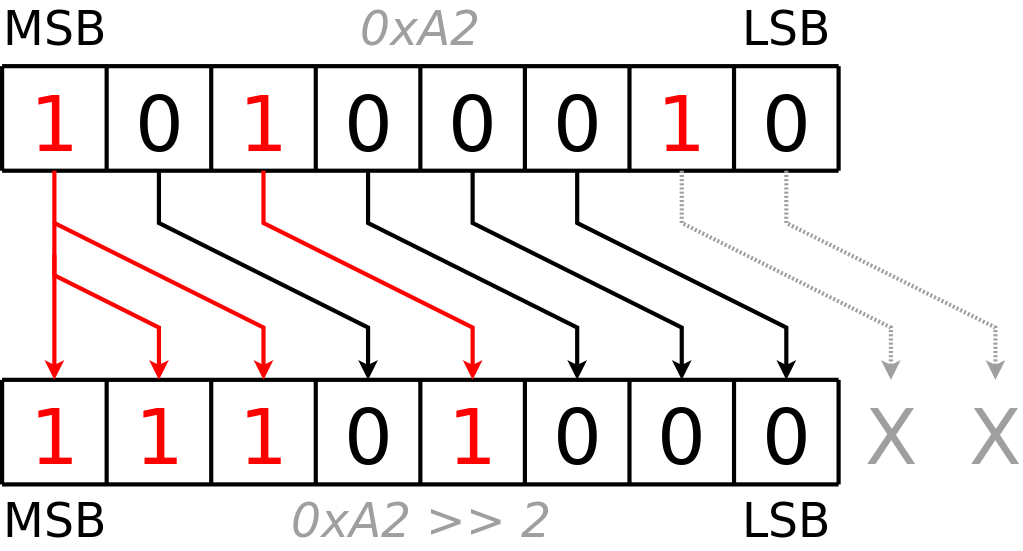
\includegraphics[width=0.7\textwidth]{./media/images/compiler/language_specification_shift_operator_right.png}
\caption{Bitweise Verschiebung einer 1.Byte Variable um 2 nach rechts}
\label{language_specification_shift_operator_right}
\end{figure}

\newpage
\subsection{Kontrollstrukturen}

Kontrollstrukturen\footnote{\url{https://de.wikipedia.org/wiki/Kontrollstruktur} } werden ben\"otigt, um den Ablauf eines Programmes zu steuern. Dies k\"onnen Verzweigungen wie auch Schleifen sein.

\subsubsection{Bedingung (if-else)}

Bedingungen\footnote{\url{https://de.wikipedia.org/wiki/Bedingte_Anweisung_und_Verzweigung}} werden genutzt, um Aktionen durchzuf\"uhren wenn eine Bedingung erf\"ullt oder nicht erf\"ullt ist. Das else ist dabei Optional, und wenn nur 1 Befehl ausgef\"uhrt wird, k\"onnen die geschwungenen Klammern weggelassen werden.

\htlParagraph{Beispiel}

\begin{lstlisting}[language=CMM]
if(a == 20)
	printf("a has the value 20");
else {
	printf("a has not the value 20");
}
\end{lstlisting}

Wenn die Variable a den Wert 20 hat wird der Text \glqq{}a has the value 20\grqq{} ausgegeben, ansonsten wird der Text \glqq{}a has not the value 20\grqq{} ausgegeben.

\begin{figure}[h]
\centering
\includegraphics[width=0.9\textwidth]{./media/images/compiler/language_specification_if_condition.png}
\caption{Flussdiagramm des Beispieles zur if-Bedingung}
\label{language_specification_if_condition}
\end{figure}

\newpage
\subsubsection{Mehrfache Verzweigung (switch-case)}

Mithilfe eines switch-case\footnote{\url{https://de.wikipedia.org/wiki/Bedingte_Anweisung_und_Verzweigung\#Erste_Form}} ist es m\"oglich, eine mehrfache Verzweigung aufzubauen, ohne mit else-if Konstrukten zu arbeiten. Es muss beachtet werden das nur konkrete Werte als Bedingung verwendet werden k\"onnen. Falls kein case-Staement mit dem \"ubergebenen Wert \"ubereinstimmt wird die default-Bedingung wenn verf\"ugbar aufgerufen.

\htlParagraph{Beispiel}

\begin{lstlisting}[language=CMM]
switch(a) {
	case 1:
		printf("a has the value 1");
		break;
	case 2:
	case 3:
		printf("a has the value 2 or 3");
		break;
	default:
		printf("a has some other value");
		break;
}
\end{lstlisting}

Es muss beachtet werden die Kontrollstruktur mit break zu verlassen, wenn der nachfolgende Code im switch nicht ausgef\"uhrt werden soll. Ansonsten kann es zu unerwarteten Ergebnissen kommen, da auch die nachfolgenden case-Statements aufgerufen werden.

\begin{figure}[h]
\centering
\includegraphics[width=0.7\textwidth]{./media/images/compiler/language_specification_switch_case.png}
\caption{M\"ogliches Flussdiagramm eines switch-case}
\label{language_specification_switch_case}
\end{figure}

\newpage
\subsubsection{while Schleife}

Die while Schleife\footnote{\url{https://de.wikipedia.org/wiki/Schleife_(Programmierung)\#While-Do-Schleife}} wird verwendet, um Anweisungen so lange zu wiederholen bis eine Bedingung nicht mehr erf\"ullt ist. Des Weiteren ist es m\"oglich, die Schleife vorzeitig zu wiederholen oder abzubrechen. 

\htlParagraph{Beispiel}

\begin{lstlisting}[language=CMM]
while(a >= 1) {
	a --;
	printf("loop: %d\n", a);
}
\end{lstlisting}

Die Schleife wird so lange durchlaufen bis die Variable $a < 1$ ist. Wenn die Variable a von Anfang an bereits kleiner 1 ist wird die Schleife nicht durchlaufen.

\begin{figure}[h]
\centering
\includegraphics[width=0.4\textwidth]{./media/images/compiler/language_specification_while.png}
\caption{m\"ogliches Flussdiagramm einer while Schleife}
\label{language_specification_while}
\end{figure}

\htlParagraph{Beispiel}

\begin{lstlisting}[language=CMM]
while(a >= 1) {
	a --;
	if(a == 3)
		continue;
	if(a == 5)
		break;
	printf("loop: %d\n", a);
}
\end{lstlisting}

Die Schleife wird so lange durchlaufen bis die Variable $a < 1$ ist. Des Weiteren wird kein Text ausgegeben falls die Variable a den Wert 3 erreicht, sondern sogleich ein erneuter Schleifendurchlauf begonnen. Falls die Variable den Wert 5 erreicht wird die Schleife vorzeitig abgebrochen.

\newpage
\subsubsection{do-while Schleife}

Die do-while Schleife\footnote{\url{https://de.wikipedia.org/wiki/Schleife_(Programmierung)\#Do-While-Schleife}} ist \"ahnlich der while Schleife, mit dem Unterschied, dass die Bedingung am Ende des Durchlaufs abgepr\"uft wird. Aus diesem Grund wird die do-while schleife mindestens 1 mal durchlaufen bevor sie verlassen wird.

Wie bei der while-Schleife ist es au\ss{}erdem m\"oglich, die Schl\"usselw\"orter \textbf{break;} und \textbf{continue;} zu verwenden, um den Schleifendurchlauf zu ver\"andern.

\htlParagraph{Beispiel}

\begin{lstlisting}[language=CMM]
do {
	a --;
	printf("loop: %d\n", a);
} while(a >= 1);
\end{lstlisting}

Die Schleife wird so lange durchlaufen, bis die Variable am Ende der Schleife $< 1$ ist. Wenn die Variable a von Anfang an bereits kleiner 1 ist wird die Schleife trotzdem 1 mal durchlaufen, bevor sie Verlassen wird.

\begin{figure}[h]
\centering
\includegraphics[width=0.4\textwidth]{./media/images/compiler/language_specification_do_while.png}
\caption{m\"ogliches Flussdiagramm einer do-while Schleife}
\label{language_specification_do_while}
\end{figure}

\newpage
\subsubsection{for Schleife}

Die for Schleife\footnote{\url{https://de.wikipedia.org/wiki/For-Schleife}} erm\"oglicht die einfache Definition von Schleifen, welche zu Beginn Werte initialisieren m\"ussen, und oder einen Schleifen-Iterator besitzen. Die for Schleife erleichtert die Definition von solchen Schleifen und k\"ummert sich um den korrekten Umgang der Schleife bei Benutzung eines \textbf{continue} oder \textbf{break}.

Zu beachten ist, dass im Gegensatz zu C keine neuen Variablen zu Beginn der Schleife erstellt werden k\"onnen. Variablendefinitionen m\"ussen immer davor erstellt werden.

Des Weiteren ist es m\"oglich, die Variableninitialisierung bzw. den Iterationsoperator leer zu lassen. Die Strichpunkte m\"ussen aber trotzdem geschrieben werden.

\htlParagraph{Beispiel}

\begin{lstlisting}[language=CMM]
for(a = 0; a <= 5; a ++) {
	printf("loop: %d\n", a);
}
\end{lstlisting}

Der Schleifeniterator wird in diesem Fall zu beginn auf 0 gesetzt, und dann nach jedem Schleifendurchlauf um 1. inkrementiert, bis die Bedingung nicht mehr erf\"ullt ist. Aus diesem Grund wird diese Schleife immer genau 6 Iterationen durchlaufen bevor sie verlassen wird. 

\begin{figure}[h]
\centering
\includegraphics[width=0.5\textwidth]{./media/images/compiler/language_specification_for.png}
\caption{m\"ogliches Flussdiagramm einer for Schleife}
\label{language_specification_for}
\end{figure}